\documentclass[12pt]{article}
\usepackage[margin=2.5cm]{geometry}
\usepackage{enumerate}
\usepackage{amsfonts}
\usepackage{amsmath}
\usepackage{fancyhdr}
\usepackage{amsmath}
\usepackage{amssymb}
\usepackage{amsthm}
\usepackage{mdframed}
\usepackage{graphicx}
\usepackage{subcaption}
\usepackage{adjustbox}
\usepackage{listings}
\usepackage{xcolor}
\usepackage{booktabs}
\usepackage[utf]{kotex}
\usepackage{hyperref}
\usepackage{accents}

\definecolor{codegreen}{rgb}{0,0.6,0}
\definecolor{codegray}{rgb}{0.5,0.5,0.5}
\definecolor{codepurple}{rgb}{0.58,0,0.82}
\definecolor{backcolour}{rgb}{0.95,0.95,0.92}

\lstdefinestyle{mystyle}{
    backgroundcolor=\color{backcolour},
    commentstyle=\color{codegreen},
    keywordstyle=\color{magenta},
    numberstyle=\tiny\color{codegray},
    stringstyle=\color{codepurple},
    basicstyle=\ttfamily\footnotesize,
    breakatwhitespace=false,
    breaklines=true,
    captionpos=b,
    keepspaces=true,
    numbers=left,
    numbersep=5pt,
    showspaces=false,
    showstringspaces=false,
    showtabs=false,
    tabsize=1
}

\lstset{style=mystyle}

\pagestyle{fancy}
\renewcommand{\headrulewidth}{0.4pt}
\lhead{CSC 343}
\rhead{Topik II 2019 Listening Test Solution}

\begin{document}
\title{Topik II 2019 Listening Test Solution}
\maketitle

\begin{enumerate}[1.]
    \item 2
    \item 1
    \item 3
    \item 3
    \item 4
    \item 2
    \item 4
    \item 4
    \item 3
    \item 2
    \item 1
    \item 2
    \item 3
    \item 2
    \item 3
    \item 3
    \item 1
    \item 2
    \item 1
    \item 2
    \item 3
    \item 1
    \item 1
    \item 1
    \item 2
    \item 3
    \item 4
    \item 2
    \item 4
    \item 4
    \item 2
    \item 4
    \item 3
    \item 4
    \item 1
    \item 3
    \item 2
    \item 4
    \item 2
    \item 1
    \item 2
    \item 4
    \item 4
    \item 2
    \item 3
    \item 1
    \item 2
    \item 4
    \item 1
    \item 1
\end{enumerate}

틀린문제: 14) - 1, 22) - 4, 30) - 3, 36) - 1, 39) - 3


\begin{center}
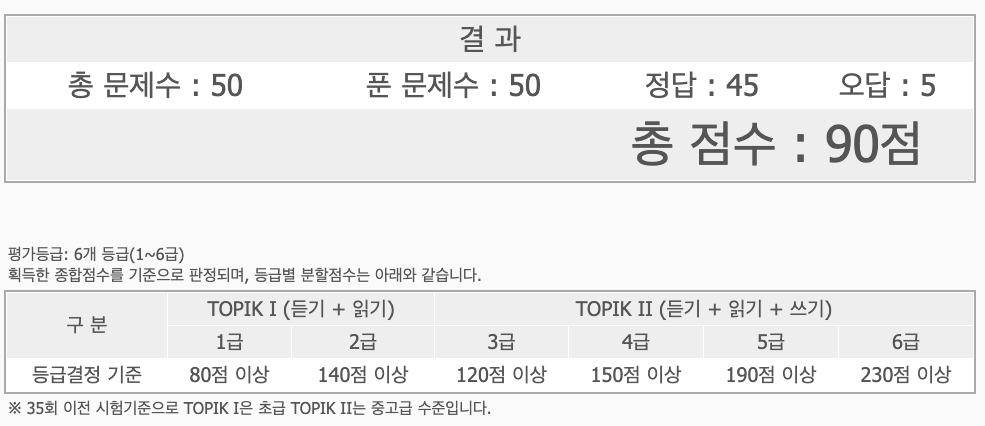
\includegraphics[width=\linewidth]{images/2019_listening_result.png}
\end{center}

\end{document}